\subsection{Baseline Models} \label{sec:baselinemodels}
This section presents the baseline model candidates and discusses the performance of each baseline candidate in turn.

\subsubsection{ResNet50 Forward Pass to Maxpooling Layer}
This model candidate is obtained by extracting the global maxpooling feature layer(\texttt{max\_pooling}) from ResNet50 pretrained on imagenet and passing input through to that layer. This was done for all image preprocessing schemes:

\begin{figure}[H]
    \centering
    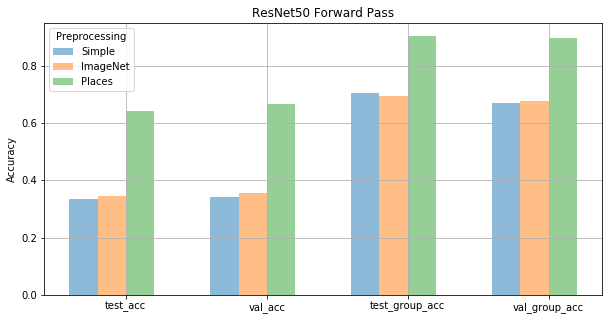
\includegraphics[scale=0.5]{pictures/plots/resnet50_fc_acc}
    \caption{Baseline performance of ResNet50}
    \label{fig:baselineresnet}
\end{figure}

\subsubsection{VGG16 Forward Pass to Fully Connected Layer}
A baseline candidate model was obtained by extracting the last fully connected(\texttt{fc\_1}) layer from VGG16 pretrained on places and passing input to through to that layer:

\begin{figure}[H]
    \centering
    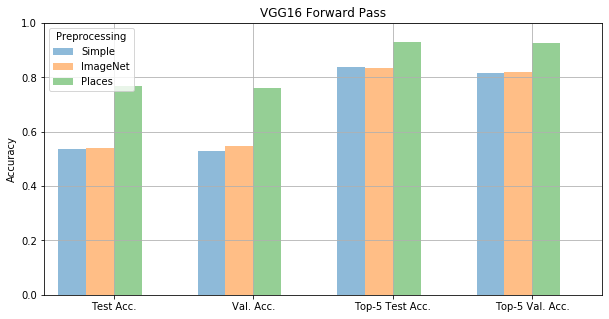
\includegraphics[scale=0.5]{pictures/plots/vgg_fc_acc}
    \caption{Baseline performance of VGG16}
    \label{fig:baselinevgg}
\end{figure}

The most performant of the baseline candidate is the VGG16 Forward Pass to \texttt{fc\_1}, achieving the significantly higher accuracy in all configurations than ResNet50 MaxPool Forward Pass. 

\begin{table}[H]
    \centering
    \resizebox{\textwidth}{!}{%
    \begin{tabular}{@{}llllll@{}}
    \toprule
    Model              & Preprocessing & Test Acc. & Val. Acc. & Top-5 Test Acc. & Top-5 Val. Acc. \\ \midrule
    ResNet50 (maxpool) & places        & 0.6438    & 0.666     & 0.904           & 0.898           \\
    VGG16 (fc\_1)      & places        & \textbf{0.769}     & 0.760               & \textbf{0.929}           & 0.927          
    \end{tabular}%
    }
\end{table}

It holds that for all candidate baseline models, the Places image preprocessing boosts accuracy by a substantial amount regardless of pretraining data.
One possible explanation for this is that the domain data of Places is significantly more in line with the target domain, that is the case for ImageNet, suggesting that subtracting the mean Places RGB-values in the target dataset provide a better input image representation for DRE19, \ref{sec:DRE19}.
